\documentclass{article}

\usepackage{arxiv}
\usepackage[UTF8]{ctex}
\usepackage[T1]{fontenc}    % use 8-bit T1 fonts
\usepackage{hyperref}       % hyperlinks
\usepackage{url}            % simple URL typesetting
\usepackage{booktabs}       % professional-quality tables
\usepackage{amsfonts}       % blackboard math symbols
\usepackage{nicefrac}       % compact symbols for 1/2, etc.
\usepackage{microtype}      % microtypography
\usepackage{lipsum}
\usepackage{graphicx}
\usepackage{cite}
\graphicspath{ {./images/}{..} }
\newcommand{\upcite}[1]{\textsuperscript{\cite{#1}}}
\title{Recsys Challenge 2023 Report}

\author{
 任子骏 \\
  PB20051046\\
  University of Science and Technology of China\\
  \texttt{renzj@mail.ustc.edu.cn} \\
  %% examples of more authors
   \And
 花昌诚 \\
  PB20030866\\
  University of Science and Technology of China\\
  \texttt{hccdmm@mail.ustc.edu.cn} \\
  %% \AND
  %% Coauthor \\
  %% Affiliation \\
  %% \texttt{email} \\
  %% \And
  %% Coauthor \\
  %% Affiliation \\
  %% \texttt{email} \\
}

\begin{document}
\maketitle

% keywords can be removed
%\keywords{First keyword \and Second keyword \and More}


\section{Introduction}

Recsys Challenge 2023作为推荐系统领域的一项竞赛,旨在探索推荐算法在大规模数据集上的性能,
为推荐系统领域的研究和应用提供创新性的解决方案。
本文旨在详细介绍我们参与Recsys Challenge 2023数据分类任务的工作,
包括问题描述、问题分析、实验方案、实验过程以及最终结果和分析。

\section{TeamWork}
\paragraph*{队伍名称} Baker street Irregulars

\paragraph*{队员信息}

\paragraph*{队员1}

姓名:花昌诚

学号: PB20030866

分工: 数据预处理、特征工程、模型设计、模型训练与调参、报告撰写

贡献: 共同设计了实验流程,构建最终模型架构,对模型进行参数调优,并将结果进行上传,负责组委会沟通与一部分的报告撰写。

\paragraph*{队员2}

姓名: 任子骏

学号: PB20051046

分工: 比赛选择、数据预处理、特征工程、模型选择、报告撰写

贡献: 共同设计了实验流程,选择比赛并对数据进行预处理,选择具有参考意义的模型与调整,负责主要报告撰写的工作。

\section{Task description and data construction}
\label{sec:headings}
在Recsys Challenge 2023中,我们的目标是提供来自 Sharechat 和 Moj 应用程序的真实广告数据集,
作为关注用户隐私的深度漏斗优化研究的基准,训练数据由过去两周的二次抽样印象/点击/安装组成,旨在预测第 15 天的安装概率。

\paragraph*{比赛链接}

\url{https://sharechat.com/recsys2023}

\subsection{问题介绍}

该数据集对应于三个月内访问 ShareChat + Moj 应用程序的大约 1000 万随机用户。 
数据集对每个用户的活动进行了采样,以生成与每个用户相对应的 10 次展示。 
目标变量是用户是否安装了应用程序。

为了代表用户,数据集提供了多种特征,\textbf{但各个特征的语义不提供,即我们不知道哪个特征是描述哪方面性质的。
同时比赛具有明确规定,为保护用户隐私,不允许推测特征的隐藏含义。}

提供的特征的隐藏含义如下:
\begin{itemize}
\item 人口统计特征:包括年龄、性别以及用户访问 Sharechat/Moj 应用程序的地理位置,用户抽样在人口统计特征上得到大致均匀的用户分布,用户的位置被哈希为 32 位以使数据匿名。
\item 内容偏好embedding:这些embedding是根据用户对 Sharechat/Moj 应用上各种非广告内容的消费情况进行训练的。
\item 应用程序亲和性embedding:这些embedding是根据用户在平台上安装的过去的应用程序进行训练的。
\item 广告分类特征:这些特征代表广告的不同特征,包括广告的大小、广告的类别等。这些特征被哈希为32位以匿名化数据。
\item 广告embedding:它们代表广告的实际视频/图像内容。
\item 计数特征:为了捕获用户和广告之间的历史交互,这些特征代表用户在不同时间窗口长度内与广告、广告商和广告商类别的交互。
\item 数据的每一行都有一个关联的数字 ID,代表向用户显示的广告印象以及它是否导致广告点击以及随后的安装。
\end{itemize}

对于生成训练和测试数据,数据集考虑了 22 个连续日期的广告投放数据。 
前 21 天构成训练数据的基础,第 22 天的数据用于生成测试数据。 
根据此基础数据创建了印象记录,这意味着用户查看了广告。 需要注意的是,就在线广告而言,用户有可能观看了广告,
然后没有点击广告,而是直接安装了底层应用程序。 此行为的含义是,我们有没有点击但有安装的记录。
数据集用两个字段(is\_clicked 和 is\_install)注释此数据,以表示用户是否进行了单击和安装。 
我们可以使用 (is\_clicked, is\_installed) 的值将整个数据集细分为四个不重叠的子集,(0, 0) 对应于既没有点击也没有安装的展示次数,
(1, 0) 对应于产生点击但未安装的展示次数,(0, 1) 对应于用户未点击但安装了应用程序的展示次数, 
(1, 1) 对应于用户执行点击并安装应用程序的展示次数。

具体数据特征如下:
每一行一共有80个特征(f\_0 to f\_79),两个标签(is\_cilcked and is\_installed)
除去RowId和Labels,一共41个类别特征,38个数值特征。
测试文件夹中有一个文件。 该文件的格式与train文件夹文件相同,但
两列(is\_clicked、is\_installed)不存在。
挑战的任务是预测测试集中记录的 is\_clicked 和 is\_installed 。
\begin{figure}[htbp]
  \centering
  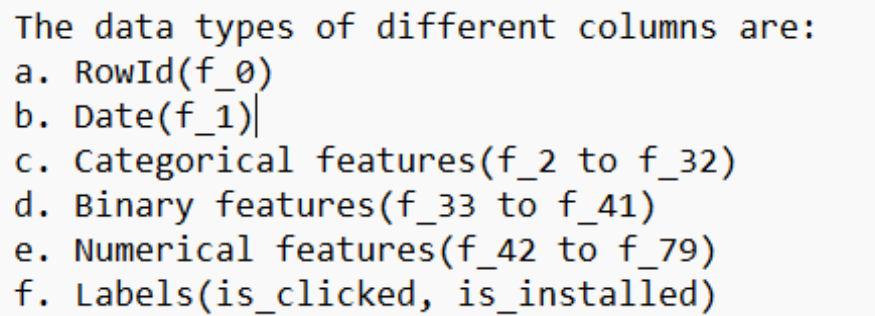
\includegraphics[scale=0.3]{data.png}
  \caption{具体数据特征}
  \label{figure3}
\end{figure}

\subsection{评价指标}
Sharechat Recsys 挑战的目的是预测用户是否会在给定的广告印象中进行安装。
这些预测用于生成一个排名,衡量平台的预期收入,然后将获胜的广告显示给用户。
由于这些预测在实际排名中使用,准确地估计概率非常重要。

为了评估任何模型的性能,我们将使用归一化交叉熵,这个指标度量了模型预测的准确性。
定义如下:

$$
Normalised-Entropy = \frac{-\frac{1}{N}\sum_{i=1}^N(\frac{1+y_i}{2}\log(p_i)+\frac{1-y_i}{2}\log(1-p_i))}{-(p\log(p)+(1-p)\log(1-p))}
$$

公式中使用的各个符号解释如下:

\begin{itemize}
  \item $N$:测试数据中的记录数量。
  \item $y_i$:测试数据中的标签,表示用户是否进行了安装(取值为 -1 或 1)。
  \item $p_i$:模型预测的用户进行安装的概率。
\end{itemize}

按照这个公式,计算基于提出的模型的每个印象的平均对数损失与基于预测了背景安装率的模型的每个印象的平均对数损失之间的比率。

提交格式: 提交文件包含三列,格式如下:

\begin{itemize}
  \item Rowld:来自测试数据文件的行号。
  \item Probability of Click given Impression:在给定印象下点击的概率。
  \item Probability of install given impression:在给定印象下进行安装的概率。
\end{itemize}

\subsection{问题分析}
本挑战是一个推荐系统问题,由于比赛具有明确规定,为保护用户隐私,我们在此不推测特征的隐藏含义。
由于需要预测测试集中记录的 is\_clicked 和 is\_installed,即安装率与点击率,我们可以将其视为一个分类问题。
由此我们寻找文献发现可以借助DeepFM模型进行训练。
DeepFM \upcite{2017arXiv170304247G}(Deep Factorization Machine)是一种用于推荐系统和点击率预测等任务的深度学习模型,
它结合了因子分解机(Factorization Machine)和神经网络的优势,以提高模型的性能和表达能力。
它在模型中融合了线性项、二阶交叉特征和深度神经网络,可以在我们任务中捕捉特征之间的复杂关系。这在我们不了解
特征具体语义上也能将特征间关系与目标对象联系起来。考虑到单个模型的泛用性能可能不是很好,我们加入XGBoost进行集成,使最终模型
较为稳健高效,同样的,XGBoost由于可以计算特征在模型中的重要性,帮助识别对预测结果影响较大的特征,也适合我们预测的分类问题。

\section{Modal Principle and Advantage}

\subsection{DeepFM}

因子分解机(Factorization Machine,简称FM)是一种用于处理高维稀疏数据的机器学习模型,
特别适用于推荐系统、广告点击率预测、自然语言处理等领域。它可以捕捉特征之间的交互关系,
包括线性和二阶交叉特征,从而能够有效地处理特征组合和高维数据。
\begin{figure}[htbp]
  \centering
  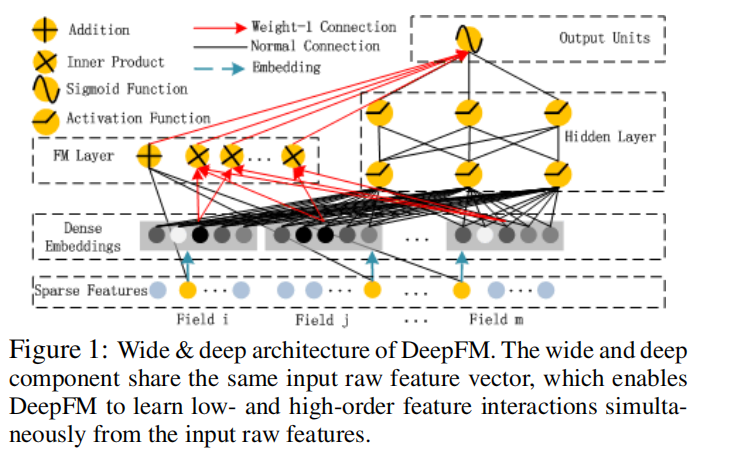
\includegraphics[scale=0.5]{DeepFM.png}
  \caption{DeepFM模型}
  \label{figure4}
\end{figure}

给定一个包含n个特征的数据集,FM的目标是学习每个特征的隐向量表示,以及特征之间的交互关系。

一阶特征: FM首先处理特征的一阶部分,即线性关系。对于一个特征$x_i$,它的线性权重表示为$w_i$。
模型将所有特征的一阶权重组合起来,得到一个线性预测部分。

二阶交叉特征: FM的核心是处理特征的二阶交叉部分,即特征之间的交互关系。为了捕捉这种交互,
FM引入了每个特征的隐向量表示$v_i$,其中$i=1,2,...,n$。对于两个特征$x_i$和$x_j$,
它们的交互项定义为$v_i \cdot v_j$,即它们隐向量的内积。这个交互项表示了特征之间的二阶交叉关系。
将所有特征的交互项相加,得到二阶交叉预测部分。

FM模型的输出可以表示为:

$$
y(x)_{FM} = w_0 + \sum_{i=1}^nw_ix_i + \sum_{i=1}^n\sum_{j=i+1}^n<v_i,v_j>x_ix_j
$$

FM主要考虑了一阶和二阶交叉特征,即特征的线性和二阶交互关系。
然而,现实世界中的数据往往包含更高阶的特征交互,这些交互无法被FM有效捕捉。

对于高阶的特征组合,很自然想到用DNN。
稀疏的onehot可以通过dense层转到隐藏层,
这样低阶特征和高阶特征的组合隐含的体现在隐藏层中。

由此,DeepFM引入了神经网络部分,在Wide\&Deep结构的基础上,使用FM取代Wide部分的LR,这样可以避免人工构造复杂的特征工程,
通过多个隐藏层来捕捉更高阶的特征交互,从而在建模复杂关系时具有优势。

在网络融合方面,DeepFM采用的是并行结构。DeepFM 预测函数为:

$$
y = sigmoid(y_{FM} + y_{DNN})
$$

\subsection{XGBoost}
XGBoost(eXtreme Gradient Boosting)是一种强大的集成机器学习算法,主要用于分类和回归任务。
它是梯度提升树(Gradient Boosting Tree)的一种改进版本,通过在每次迭代中引入正则化和优化技巧,使模型更加稳健和高效。

XGBoost采用集成学习的思想,初始化一个初始预测模型,计算损失函数的负梯度(残差),以及损失函数的二阶导数(海森矩阵)。
在每次迭代中,根据负梯度拟合一个决策树模型,以学习样本的残差。将新建的决策树模型添加到现有模型中,更新预测结果。
基于梯度提升框架,重复以上步骤,每次迭代都在前一轮模型的基础上继续改进。每个新的决策树都试图纠正前一轮模型的错误。
这种迭代的方式可以逐步改进模型的拟合能力。
最后通过加权平均或投票等方式,通过组合多个弱学习器(决策树)来构建一个强学习器,
将多个决策树组合成最终的预测模型,从而提高模型的预测性能。

\section{Experiment and Discussion}

\subsection{代码结构}

所有必要代码由args、dataset、DeepFM、evaluation、result\_mean、main六部分组成,具体文件说明如下:
\begin{itemize}
  \item args.py:设置公共的参数;
  \item dataset.py:处理数据集,设置获取单个样本数据的格式;
  \item DeepFM.py:网络结构的设置、模型训练、保存结果,核心文件;
  \item evaluation.py:官方给出的评估代码
  \item result\_mean.py:将两个模型得到的结果进行平均取值
  \item main.py与main.ipynb:前者运行DeepFM模型的主函数,后者包括开始的数据分析和XGBoost模型的参数设置
\end{itemize}

\subsection{数据预处理}

数据预处理由dataset.py文件进行。

首先读取训练集和测试集数据,并进行特征和标签的分离。由于训练集文件过多,使用glob进行读取,测试集文件直接读取。
由于训练集文件特征冗杂,还需对特征进行抽取选用和编码,从而划分训练集与验证集。
\begin{figure}[htbp]
  \centering
  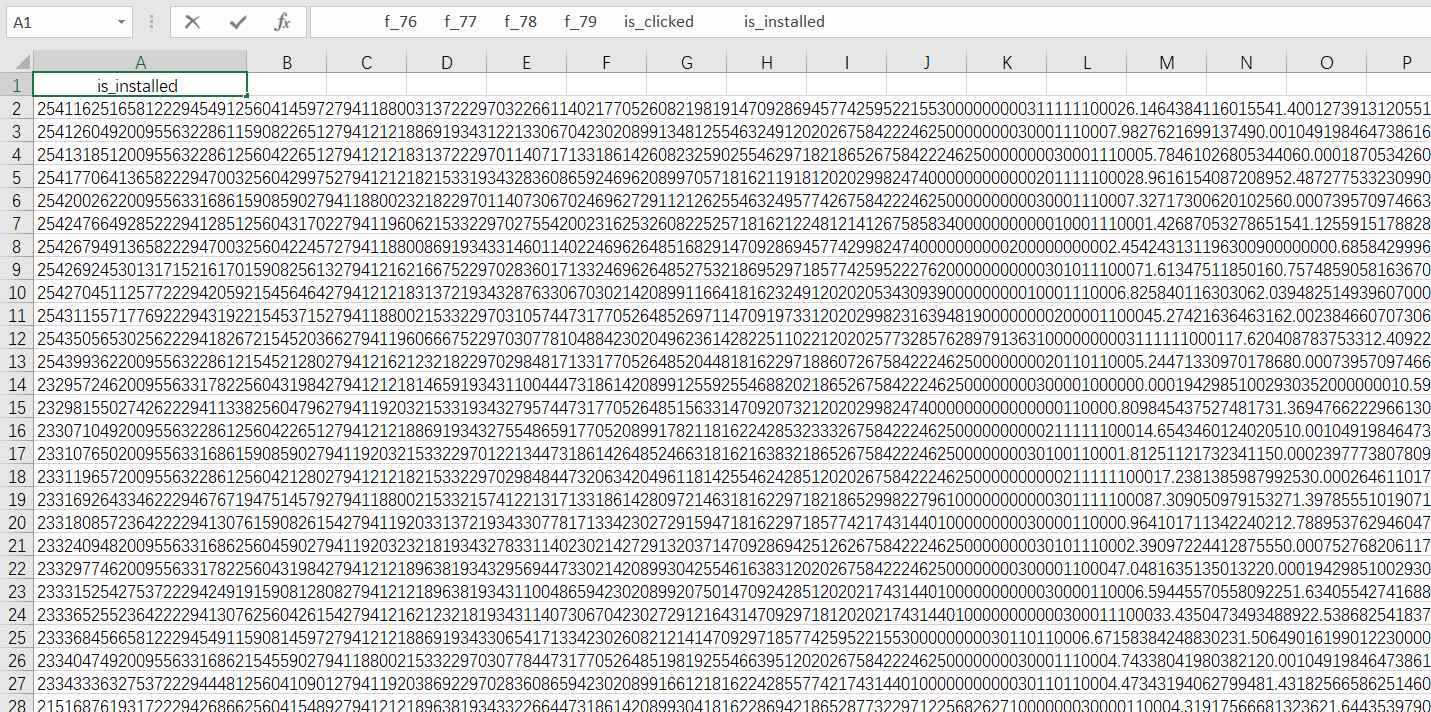
\includegraphics[scale=0.3]{rawdata.png}
  \caption{具体数据}
  \label{figure6}
\end{figure}

随后,定义数据加载类RecSysDataset初始化数据集,根据索引获取数据,方便后续进行分析。

因为是一个时间周期下预测用户未来一天的安装概率,因此我们分析不同天数的样本总的点击率和安装
率,如图所示:

\begin{figure}[htbp]
  \centering
  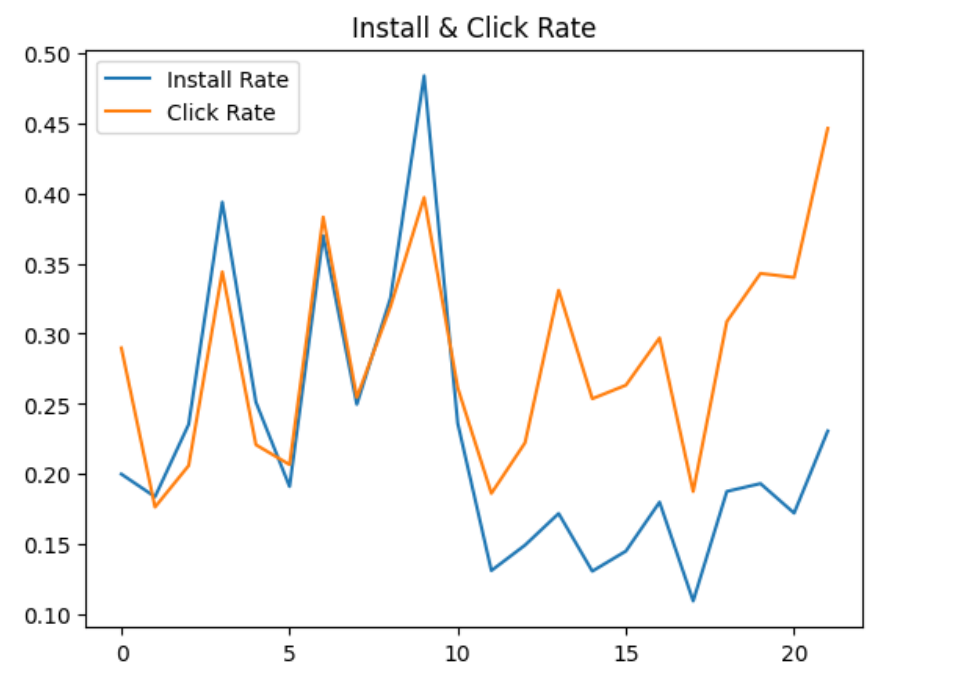
\includegraphics[scale=0.3]{Install.png}
  \caption{样本点击率与安装率}
  \label{figure7}
\end{figure}

此外,我们还统计特征每列和y\_install之间的相关性,方便后续对特征进行筛选。
需注意,特征筛选过程不是一蹴而就的,是根据实验结果一步步优化得到的,
在后面将会有详细论述。

\subsection{初步尝试}

我们对于DeepFM的构建主要根据GitHub前人的代码,同时结合对问题自身特点的理解,加入了自己的修改。以下列举我们所加入的一些重要代码设置:

\begin{itemize}
  \item 参数设置:我们将预先求得的类别特征信息、数值特征标志、预测点击或安装等必要参数放入args.py中,不用每次都从命令行输入,运行时进行修改即可。
  \item 实验记录:记录每次训练的loss和accuracy(因为该任务样本量较大,不是将全部样本训练完后得到其loss,而是设置一个超参print\_every,
  每经过这么多次batch之后记录训练loss和accuracy),根据预测标签的不同写入txt文件中。
  \item 初步预处理:对离散特征进行重新编码和归一化,此时训练集和测试集放一起同步处理。
  \item 可视化:将参数的设置全部放在main.py中方便调整,同时lab\_id记录每次实验的结果和图像。
\end{itemize}

保持基本的DeepFM模型不变,我们主要思路是调整网络结构的参数、初始数据的处理等。

一开始进行模型的调参,关注的模型参数分别如下所述:

- embedding\_size:将类别特征进行映射的大小

- hidden\_dims:网络结构,基本的前馈神经网络每层神经元数

- dropout:经过每层网络后dropout的概率,默认全部相同

- 还有比如验证集的大小、早停策略paience的设置

- batch\_size:每个batch的样本大小

\begin{figure}[htbp]
  \centering
  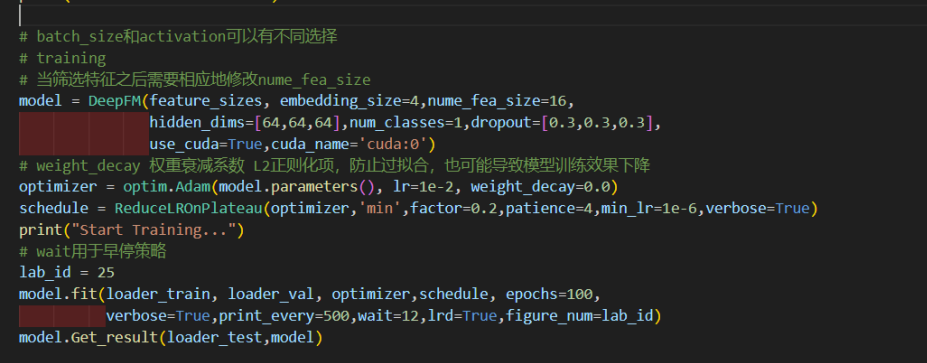
\includegraphics[scale=0.3]{arg1.png}
  \caption{参数设置}
  \label{figure8}
\end{figure}

经过调参最明显的体验就是变化规律并不明显,总结原因是因为超参数对结果的影响并没有那么显著,无法排除偶然因素的干扰,
也因为测试集的情况是未来某一天的数据,其分布完全无法预知,所以并没有找到一定最优的超参数,
但是基本确定了较为合适的超参。举例来说,比如embedding\_size=2/4较为合适,因为类别特征唯一值个数也是2/4居多,因此符合实验结果和主观判断。

为了加快模型的训练,并不是在每个epoch全部样本训练之后才进行train\_loss和val\_loss的计算,
而是在训练过程中经过给定次数个batch即计算一次,然后判断要不要早停,这样做的好处是训练epoch数会减少,
坏处是可能与样本的分布有关导致过早早停,在后期更改了该设置加大训练时长后,指标有所提升。

\subsection{特征选择}

当调参陷入僵局之后,需要从别的方面来寻求进一步指标的提升,这时候我们开始思考将特征不加筛选一股脑的丢进去是否合理,结论是显然对特征进行初步的筛选是有必要的。

\begin{figure}[htbp]
  \centering
  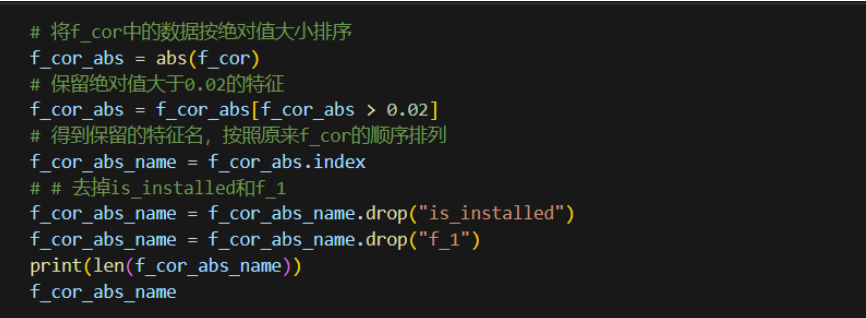
\includegraphics[scale=0.3]{feature.png}
  \caption{特征选择}
  \label{figure9}
\end{figure}

我们将数值特征和类别特征不作区分,统一计算它们和标签的相关性,同时设置不同的相关系数阈值,
比如只选择相关性绝对值>0.02的特征放入网络训练,在经过几次不同阈值的尝试之后,我们发现选择特征不同对结果会产生明显的影响,
因此在选择表现最好的阈值之后指标也提升了不少;

同时因为该任务并未对每个特征的语义阐明,我们无法根据个人的主观经验或是背景
知识手动选取特征或是进行特征组合,只能分析数据的分布特点做一定的推测来选取特征尝试。


\subsection{模型集成}

在DeepFM模型经过调参和不同尝试取得了还算不错的效果且提升不明显之后,我们想要尝试加入一个传统
的机器学习模型进行两个模型的集成来获得结果,但是该模型并未花很多时间去调整。基本思路是直接
调用xgboost库的XGBClassifier来处理该任务,初步试探了不同的特征选取和参数设置之后得到了实验
结果。

简单的想法是将两个模型得到的预测概率做一个平均作为最终结果,同时也尝试了不同的比重提交查看排行榜分数,
发现简单平均的效果最好,因此模型的集成只是将结果求平均,排名又上升了一些之后即结束了本次比赛。

由于在比赛过程中我们测试的参数组过多,不方便一一列举,下面展示训练过程中保存的一次loss截图(示例)
\begin{figure}[htbp]
  \centering
  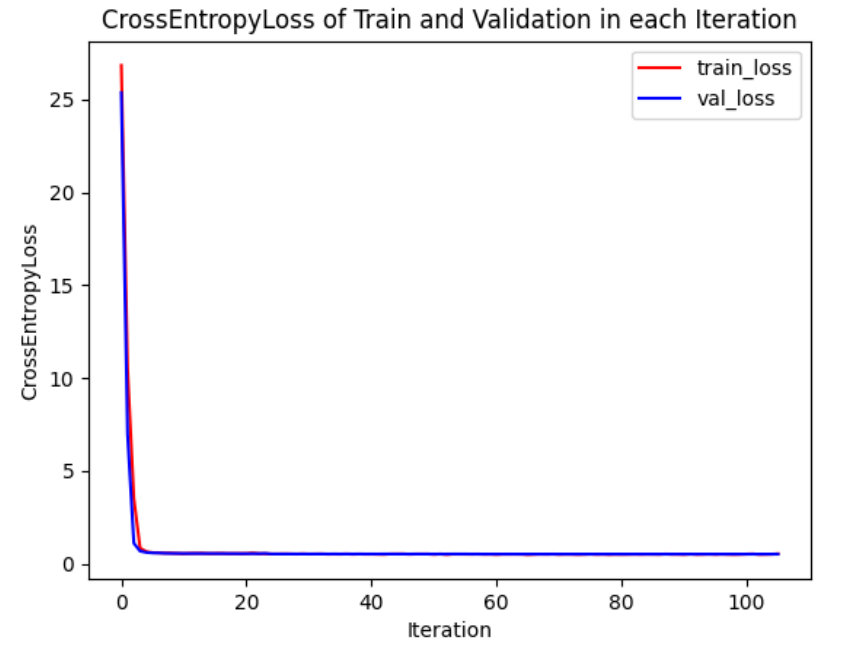
\includegraphics[scale=0.3]{loss.png}
  \caption{loss曲线}
  \label{figure11}
\end{figure}

\subsection{其他尝试}

在官方公布测试集的评估函数之后,猜想不同的损失函数的设置是否也会对结果产生影响,
比如因为数据集的正负样本比例是有差异的,如果尝试对正样本的误差给予更多关注,
即如果用户标签是会下载而模型预测为不下载,那么分类错误,将该误差放大以提高对样本的关注,
通过设置正负样本的权重实现。从结果来看确实发生了较大变化,但是是往坏的趋势变化,因此该尝试失败。

\begin{figure}[htbp]
  \centering
  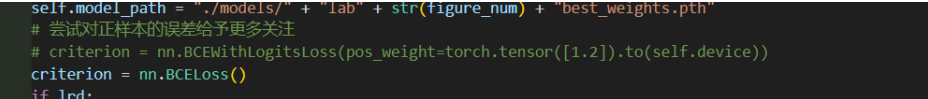
\includegraphics[scale=0.3]{try1.png}
  \caption{关注偏置}
  \label{figure10}
\end{figure}
\clearpage
\section{Results}
我们在Recsys Challenge 2023中得分以及排名如图所示。(注:本比赛Leaderboard有两个,我们的排名位于Academia上)

\begin{figure}[htbp]
  \centering
  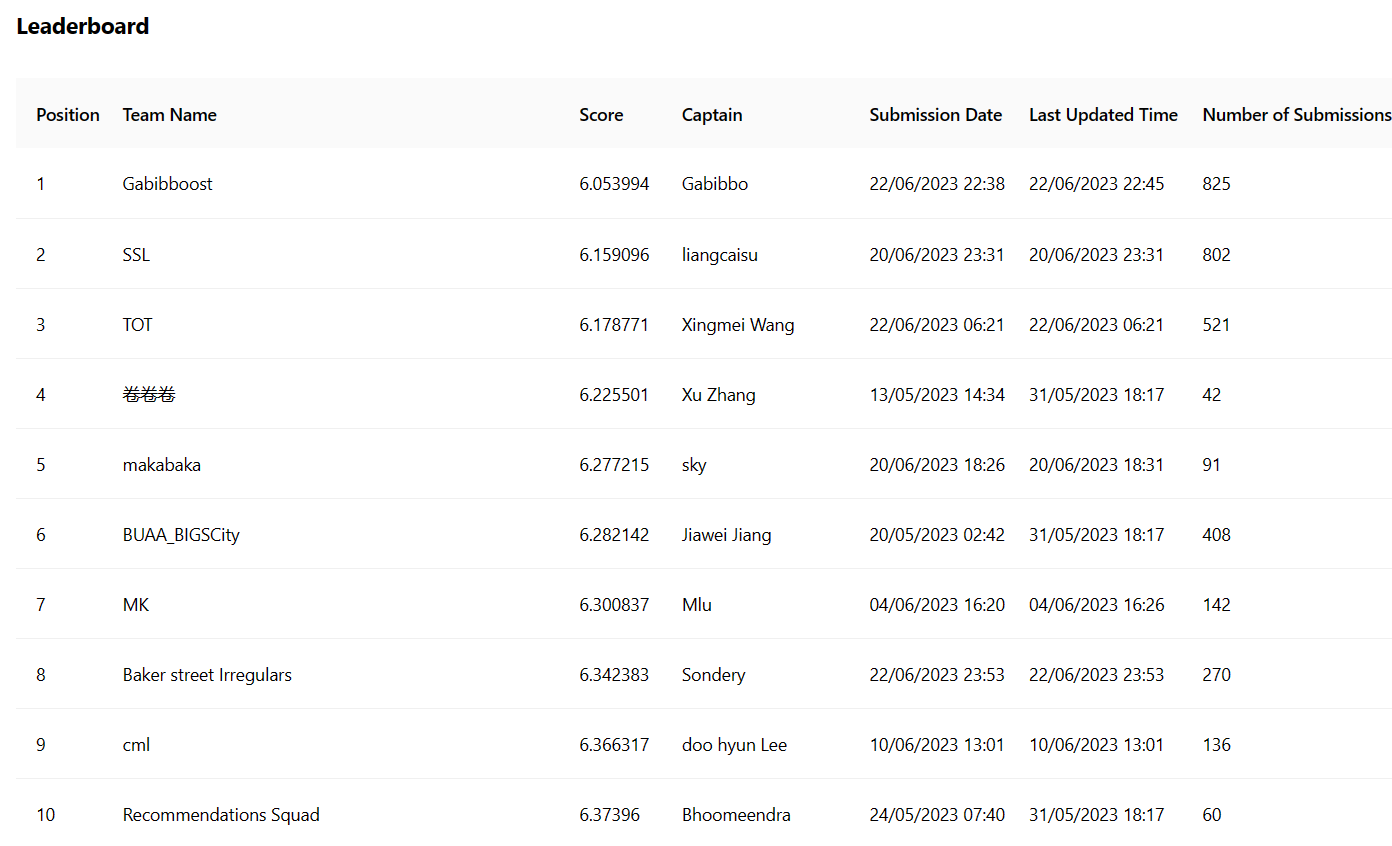
\includegraphics[scale=0.3]{results.png}
  \caption{Leaderboard Academia Rank}
  \label{figure5}
\end{figure}

我们队伍的最终模型得分为6.342383,排名8/54。


\bibliographystyle{ieeetr}
\bibliography{ref}


\end{document}
